
\documentclass{article}
\usepackage{pgfplots}
\usepackage{pgfplotstable}
\usepackage{tikz}
\pgfplotsset{compat=1.8}
\begin{document}
    \begin{figure*}[t]
        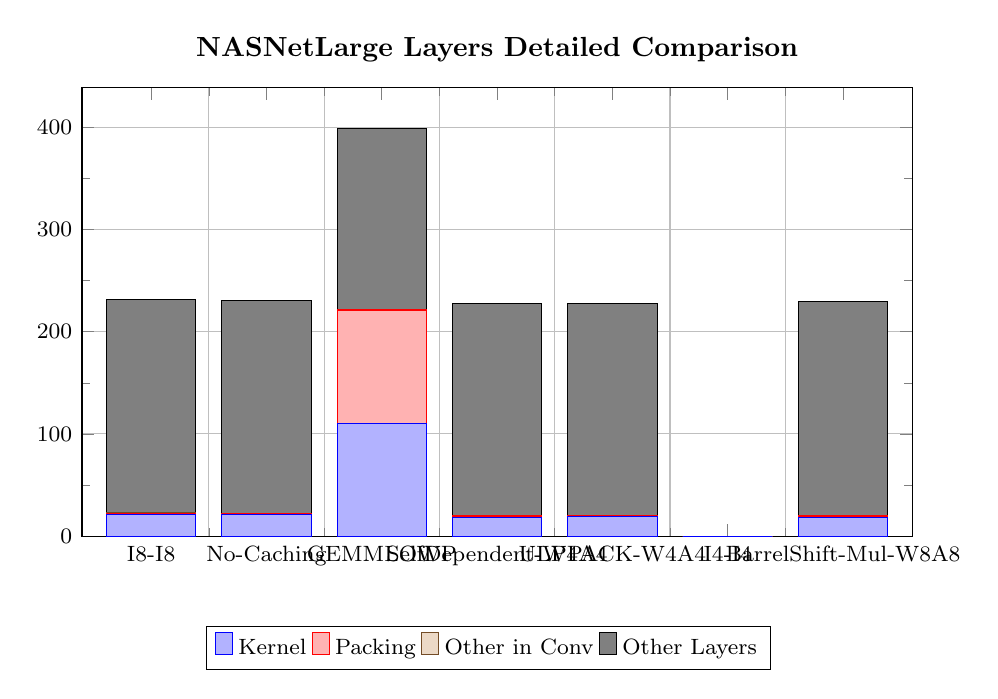
\begin{tikzpicture}
            \begin{axis}[
                ybar stacked,
                ymin=0.0,
                width=\linewidth,
                height=\axisdefaultheight,
                tick label style={font=\footnotesize},
                legend style={font=\tiny},
                label style={font=\footnotesize},
                symbolic x coords={I8-I8, No-Caching, GEMMLOWP, SelfDependent-W4A4, ULPPACK-W4A4, I4-I4, BarrelShift-Mul-W8A8},
                xtick=data,
                % ytick={0.60,0.80,1.0,1.2,1.4,1.6,1.8,2.0,2.2,2.4,2.6,2.8,3.0},
                align={center},
                bar width=7.5ex,
                legend columns=7,
                legend style={at={(0.49,-0.2)},anchor=north,font=\footnotesize},
                title=\textbf{NASNetLarge Layers Detailed Comparison},
                ymajorgrids,
                xminorgrids = true,
                minor tick num=1
                ]
                \addplot coordinates { (I8-I8,21.58) (No-Caching,21.61) (GEMMLOWP,110.61) (SelfDependent-W4A4,18.67) (ULPPACK-W4A4,19.17) (I4-I4,0.00) (BarrelShift-Mul-W8A8,18.71) };
                \addplot coordinates { (I8-I8,1.02) (No-Caching,0.92) (GEMMLOWP,110.61) (SelfDependent-W4A4,1.05) (ULPPACK-W4A4,0.98) (I4-I4,0.00) (BarrelShift-Mul-W8A8,1.06) };
                \addplot coordinates { (I8-I8,0.05) (No-Caching,0.05) (GEMMLOWP,0.03) (SelfDependent-W4A4,0.05) (ULPPACK-W4A4,0.05) (I4-I4,0.00) (BarrelShift-Mul-W8A8,0.05) };
                \addplot coordinates { (I8-I8,208.96) (No-Caching,208.11) (GEMMLOWP,177.30) (SelfDependent-W4A4,208.15) (ULPPACK-W4A4,207.68) (I4-I4,0.00) (BarrelShift-Mul-W8A8,209.97) };
                \legend{
                    Kernel,
                    Packing,
                    Other in Conv,
                    Other Layers,
                };
            \end{axis}
        \end{tikzpicture}
    \end{figure*}
\end{document}
